\documentclass{article}
% Change "article" to "report" to get rid of page number on title page
\usepackage{amsmath,amsfonts,amsthm,amssymb}
\usepackage{setspace}
\usepackage{Tabbing}
\usepackage{fancyhdr}
\usepackage{lastpage}
\usepackage{extramarks}
\usepackage{url}
\usepackage{chngpage}
\usepackage{longtable}
\usepackage{soul,color}
\usepackage{graphicx,float,wrapfig}
\usepackage{enumitem}
\usepackage{morefloats}
\usepackage{multirow}
\usepackage{multicol}
\usepackage{indentfirst}
\usepackage{lscape}
\usepackage{pdflscape}
\usepackage{natbib}
\usepackage[toc,page]{appendix}
\providecommand{\e}[1]{\ensuremath{\times 10^{#1} \times}}

% In case you need to adjust margins:
\topmargin=-0.45in      % used for overleaf
%\topmargin=0.25in      % used for mac
\evensidemargin=0in     %
\oddsidemargin=0in      %
\textwidth=6.5in        %
%\textheight=9.75in       % used for mac
\textheight=9.25in       % used for overleaf
\headsep=0.25in         %

% Homework Specific Information
\newcommand{\hmwkTitle}{Final Project Report}
\newcommand{\hmwkDueDate}{Friday,\ December\  7,\ 2018}
\newcommand{\hmwkClass}{Final Project}
\newcommand{\hmwkClassTime}{CSE 597}
\newcommand{\hmwkAuthorName}{Yueze Tan}
\newcommand{\hmwkNames}{yut75}

% Setup the header and footer
\pagestyle{fancy}
\lhead{\hmwkNames}
\rhead{\hmwkClassTime: \hmwkTitle} 
\cfoot{Page\ \thepage\ of\ \pageref{LastPage}}
\renewcommand\headrulewidth{0.4pt}
\renewcommand\footrulewidth{0.4pt}

%%%%%%%%%%%%%%%%%%%%%%%%%%%%%%%%%%%%%%%%%%%%%%%%%%%%%%%%%%%%%
% Make title

\title{\vspace{2in}\textmd{\textbf{\hmwkClass}} \\
\vspace{0.1in}\large{ \hmwkClassTime}\vspace{3in}}

\author{\textbf{\hmwkAuthorName} \\ \vspace{0.1in}
\hmwkDueDate }
\date{} % to take away today's date

%%%%%%%%%%%%%%%%%%%%%%%%%%%%%%%%%%%%%%%%%%%%%%%%%%%%%%%%%%%%%

\begin{document}
\begin{spacing}{1.1}
\maketitle

\newpage
\section*{Abstract}


Discussed in this report is the numerical approaches to solving of modified electrostatic Poisson equation with shielding effect that has a characteristic shielding length (known as Debye length). We first introduce the equation $(\nabla^2 - \lambda_D^{-2})\Phi =-\rho / \varepsilon$ along with its physical meanings, then describe the discretization method. Direct solver (partial-pivoting LU decomposition) and iterative solver (Jacobi method) are both introduced and compared.

The iterative solver is then parallelized with MPI. The justification of the parallelization method and the profiling of the code are also discussed in this report, after which we show the scaling results for multi-core calculations. We also link the code to MKL library, elevating its performance, which is also discussed with profiling and scaling results. Possible directions for next step of optimization is also discussed.

\section{Problem of Interest}

The problem is related with solving the electrostatic equation in a system with free charges and shielding effects, typical examples of which would be plasma or electrolytes. From Boltzmann's distribution we can obtain the equation describing the shielded, or compensated field:
\[(\nabla^2 - \lambda_D^{-2})\Phi=-\frac{\rho}{\varepsilon},\]
in which $\Phi$ is the electric potential, $\rho$ is the charge density which is contributed by other effects than shielding, like charge density induced by inhomogeneous distribution of polarization in a dielectric matter, and $\varepsilon$ is permittivity of the system.

For free-moving charge is common in various physical systems, charge compensation and spontaneous shielding effect could be widely observed in different kinds of condensed systems. In order to get a more accurate solution in these systems, solving the electrostatic equation with Debye length term is a necessary step. The distribution of electric potential is an interested topic in various fields, like materials science, condensed matter physics and chemical engineering, where electrolytes are extensively discussed.

Other numerical methods could also be applied to solve this problem, as what could be done for many other different types of PDEs. One possible way is using finite-element method (FEM), in which we discretize the system into piecewise functions, and then transform the problem into a integration form:
\[\int_V\left[(\nabla^2-\lambda_D^{-2})\Phi+\frac{\rho}{\varepsilon}\right]v_i\;\mathrm{d}V=0,\]
in which $v_i$ is a set of specially chosen functions to simplify the integrations.

Or we can use fast Fourier transform (FFT) to solve this problem, by transforming the original field into Fourier spectrum and then solve the algebraic equation in the frequency domain:
\[(k_1^2+k_2^2+k_3^3-\lambda_D^{-2})\Phi^K=-\frac{\rho^K}{\varepsilon},\]
and by taking inverse FFT (IFFT) on the spectrum we can get the field in real space. Such a method has already been used to solve the conventional electrostatic problem in phase-field models, see \citep{li2002}.

It might be of the readers' interest that this problem has an analytical solution, which is based on its Green function:
\[ \Phi(\mathbf{r}) =
\int _V \frac{\rho(\mathbf{r'}) (\mathbf{r} - \mathbf{r'}) \exp(|\mathbf{r} - \mathbf{r'}| / \lambda_D)}{|\mathbf{r} - \mathbf{r'}|^3} \;\mathrm{d}^3 \mathbf{r'} +
\oint _{\partial V} \frac{\sigma(\mathbf{r'}) (\mathbf{r} - \mathbf{r'}) \exp(|\mathbf{r} - \mathbf{r'}| / \lambda_D)}{|\mathbf{r} - \mathbf{r'}|^3} \;\mathrm{d} S.\]
Basically, this solution is a modified version of the regular electrostatic solution for Poisson equation, but equipped with an exponentially decaying factor so the electric potential drops much faster, which is what we are expecting from a shielding effect.

However, carrying out such an integration is practically unfavourable for most cases, as the time consumption is not satisfying, and precision of numerical solution is also suspicious since the expression to be integrated is divergent at $\mathbf{r} = \mathbf{r'}$. Besides, for most cases the boundary condition is of Dirichlet's type, which means $\sigma(\mathbf{r'})$ is unknown on the boundary of the integrated region. Therefore, a numerical way of solving the original PDE is practically more favourable.

\subsection{Numerical Set-up}

We discretize the original system using finite difference method with a uniform meshgrid, so that for a field $f(x,y,z)$, its discretized form will be
\[f_{i,j,k}=f(i\Delta x, j\Delta y, k\Delta z).\]
Hereafter, we set the discretization step as $\Delta x = \Delta y = \Delta z = 1$ nm.
Using Taylor's expansion,
\[f(x+\Delta x) = f(x)+\frac{\partial f(x)}{\partial x}\Delta x+\frac{1}{2!}\frac{\partial ^2 f(x)}{\partial x^2} (\Delta x)^2+\dots ,\]
\[f(x-\Delta x) = f(x)-\frac{\partial f(x)}{\partial x}\Delta x+\frac{1}{2!}\frac{\partial ^2 f(x)}{\partial x^2} (\Delta x)^2-\dots .\]
By adding them up and deprecating terms higher than 3rd order, we have
\[\frac{\partial^2 f(x)}{\partial x^2}\approx\frac{f(x+\Delta x)+f(x-\Delta x)-2f(x)}{(\Delta x)^2}.\]
Therefore the original equation could now be discretized as
\[\frac{\Phi_{i+1,j,k}+\Phi_{i-1,j,k}-2\Phi_{i,j,k}}{(\Delta x)^2}+
\frac{\Phi_{i,j+1,k}+\Phi_{i,j-1,k}-2\Phi_{i,j,k}}{(\Delta y)^2}+
\frac{\Phi_{i,j,k+1}+\Phi_{i,j,k-1}-2\Phi_{i,j,k}}{(\Delta z)^2}-
\lambda_D^{-2}\Phi_{i,j,k}
=-\frac{\rho_{i,j,k}}{\varepsilon}.\]

By arranging the values of a field in a vector,
\[\mathbf{f}=\left[\begin{matrix}f_{0,0,0} \\ \vdots \\ f_{i-1,j,k} \\ f_{i,j,k} \\ f_{i+1,j,k} \\ \vdots \\ f_{i,j+1,k} \\ \vdots \\ f_{i,j,k+1} \\ \vdots\end{matrix}\right],\]
we can rewrite the discretized equation in matrix form,
\[\mathbf{A\Phi}=-\frac{1}{\varepsilon}\mathbf{\rho},\]
where
\[\mathbf{A}=
\left[\begin{matrix}
\ddots & & \ddots & & \ddots & \ddots & \ddots\\
\dots & \frac{1}{(\Delta z)^2} & \dots & \frac{1}{(\Delta y)^2} & \dots & \frac{1}{(\Delta x)^2} & C & \frac{1}{(\Delta x)^2} & \dots\\
& & \ddots & & \ddots & & \ddots & \ddots & \ddots
\end{matrix}\right]\]
with
\[C:=-\left[\frac{2}{(\Delta x)^2}+\frac{2}{(\Delta y)^2}+\frac{2}{(\Delta z)^2}+\lambda_D^{-2}\right].\]
Each row/column of matrix $\mathbf{A}$ has as most 7 non-zero elements, which means this matrix could be quite sparse for large number of grid points. Seen from the form of coefficients, it is also not hard to discover that this matrix is diagonally dominant, which makes it possible to be iteratively solved with Jacobi's method. However, in real applications, the most commonly seen situation is that the boundary of the system is of Dirichlet's type, because free charge in the surroundings would attach to the surface of the system, leading to a compensation effect on the surfaces. Therefore, electric potential for the surface layer would be assigned as 0, and only a trimmed version of problem with the central $(n_x-2)(n_y-2)(n_z-2)$ points will be included in the computation, however for large problems this is of the same order of magnitude for the original problem, hence we are not distinguishing between them hereafter. For a real product sized problem, the number of grids $n_x$, $n_y$ and $n_z$ could be several tens to hundreds ($10^2$), and the total number of $n$ could be at a level of $10^6$. However, this leads to an acceptable computation time for direct solver, therefore in the following discussions we always use $n_x$, $n_y$ and $n_z$ for at most 20 for test cases.

The $\mathbf{b}$ vector is  $-\mathbf{\rho}/\varepsilon$, where $\mathbf{\rho}$ is the discretized externally applied charge density, which is a field that is already known.

\section{Solvers}

\subsection{Direct Solver}

In solving this problem, partial-pivoting LU decomposition solver is used. This solver decomposes the target matrix $\mathbf{A}$ with switching of rows in the process of decomposing, so that
\[\mathbf{PA = LU},\]
in order to avoid 0 (or very close to zero) diagonal elements in the process of LU decomposition. To get the solution, we simply use
\[\mathbf{x}=(\mathbf{PA})^{-1}(\mathbf{Pb})=\mathbf{U}^{-1}\mathbf{L}^{-1}\mathbf{Pb}.\]

In real application scenes, solving of electric field is very likely to be carried out for hundreds/thousands of times during the process of solving an entire problem. That makes matrix decomposition an appealing method compared to Gauss elimination method.

The optimization flags used are:
\begin{itemize}
    \item \texttt{-O2} - Enabling the optimizations while not inducing a significant increasing of compiling time. The execution time is rather similar for \texttt{-O2} and \texttt{-O3}. For example, time for PLU decomposition is around 48170 ms for \texttt{-O2}, while for \texttt{-O3} it is 47920 ms, with only a negligible speed up, and the iterative solver even gets slightly slower with \texttt{-O3}. On the other hand, compilation time will rise from around 2s with \texttt{-O2} to around 3s with \texttt{-O3}. Though these values are small now, we can expect a rising of several tens of percent for compilation time for larger programs, which is typically not favourable.
    \item \texttt{-mfma} - Enabling fused add-multiplication in order to speed up the index computations and possibly some algebraic operations.
    \item \texttt{-mavx} - Enabling the optimizations for vectorized data to speed-up matrix operations.
\end{itemize}

For the tests, we assign the expected size of the system from the input file (filename served as the argument of program), which contains 30 randomly distributed charged points. To modify the Debye lengths, please modify the main program and recompile. We use a $20\times 20\times 10$ system as test case.

The test results could be seen from the on-screen outputs. There is a copy in the output folder named \texttt{trackinfo.txt}. From this file we can see that for a $20\times 20\times 10$ problem, time consumption for matrix decomposition is around 30 s, and more than 20 s for finding the inverse matrices of $\mathbf{L}$ and $\mathbf{U}$. Direct solver using $\mathbf{P}$, $\mathbf{L}$ and $\mathbf{U}$ to find $\mathbf{x}$ (in our case, $\mathbf{\Phi}$) runs much faster, using only 40 ms and 70 ms respectively. Basically, using back-fill type methods will cost less time than multiplying the inverse matrix directly for this test case. This is important since back-fill type method does not only behaves fast, but is actually more numerical stable, thus should be the prior choice for this problem.

The memory allocated for the test case is around 160 MB for saving the matrices $\mathbf{P}$, $\mathbf{L}$ and $\mathbf{U}$, and around another 60 MB to save the original matrix $\mathbf{A}$. As the dimension of matrix is actually $18\times 18\times 8 = 2592$, the size of a single matrix will be around $(2600)^2\times 8/10^6\approx 54$ MB, which is rather close to the measurements. On the other hand, saving of such a field would only cost $20\times 20\times 10\times 8/10^3 = 32$ KB, which is much smaller than the cost of saving the matrix. Each inverse matrix costs around 50 MB then, in the next step. These consists of almost all the spatial occupations of the program.

For a production size program, the solver could be used to solve a $100\times 100\times 20$ problem, which means $N'=50N$, and the matrix, if possible, could be 2500 times larger than currently constructed. That will be 400 GB for the $\mathbf{P}$, $\mathbf{L}$ and $\mathbf{U}$ matrices, hardly to be saved in memory. As this is a highly sparsed matrix with only 7 non-zero elements in each row, it would be necessary to use sparse matrix for a real production problem.

Finally, it is worth noting that direct solvers could be incredibly slow for solving the 3D fields when using Gauss elimination or decomposition methods, as the size of matrix $\mathbf{A}$ growth at a speed of $O(N^2)=O(n_x^6)$ with regard to the numbers of grids $n_x$ on one direction, making the time consumption of decomposition grows in $O(N^3)=O(n_x^9)$. This makes things worse than the case of memory consumption, as that would only grow in $O(n_x^6)$. For a $100\times 100\times 20$ system, it is expected to cost over 1000 hours (!) for the matrix decomposition, which is even more unacceptable. Applying specifically designed algorithms on sparse matrix could also help resolve this problem.

\subsection{Iterative Solver}

Iterative solver used in this project is Jacobi's iterative solver, which calculates the value of next step based totally on known values:
\[\Phi^{n+1}_{i,j,k} = \frac{\frac{1}{(\Delta x)^2}(\Phi^{n}_{i-1,j,k}+\Phi^{n}_{i+1,j,k})+\frac{1}{(\Delta y)^2}(\Phi^{n}_{i,j-1,k}+\Phi^{n}_{i,j+1,k})+\frac{1}{(\Delta z)^2}(\Phi^{n}_{i,j,k-1}+\Phi^{n}_{i,j,k+1})+\rho/\varepsilon}{\frac{2}{(\Delta x)^2}+\frac{2}{(\Delta y)^2}+\frac{2}{(\Delta z)^2}+\lambda_D^{-2}}.\]

Actual calculations are carried out in matrix form of this equation, rather than update element-by-element. This solver is selected based on the consideration on both convergence and compatibility with further parallelization. Note that Jacobi method is unconditionally convergent, therefore no extra criterion is in need of specification. Residual is selected as maximum of difference between two steps, which is easy to compute, and ensures that error in electric potential is controlled in a specific range for every grid point in the system. As this solver shares the same entrance with the direct solver in the main function, please check the direct solver chapter for the optimization flags.

The residual is selected to make sure the error of electric potential is controlled under a specific threshold, and the limit is dependent of the problem requirement. Here, we arbitrarily choose $10^{-10}$ as the threshold, which makes the potential accuracy higher than $10^{-10}$ V. However, in most cases, $10^{-5}$ is already a good threshold.

Time for the test case with the same size in the previous chapter of direct solver is much faster for the iterative solvers.

The convergence of the solvers are shown in the figure below.

\begin{figure}[H]
\centering
    \begin{subfigure}
      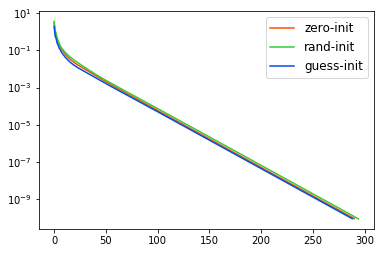
\includegraphics[width=0.4\linewidth]{output/iterative-error.png}
      \label{fig-convergence}
  \end{subfigure}
  \begin{subfigure}
      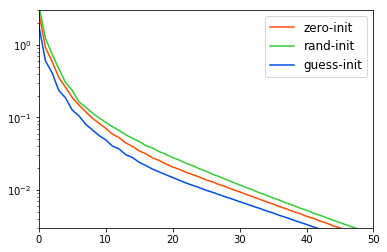
\includegraphics[width=0.4\linewidth]{output/iterative-error-magnified.png}
      \label{fig-convergence-magnified}
  \end{subfigure}
  \caption{Convergence curve of iterative solver. Horizontal axes indicates iteration cycle number. Vertical axes is the maximum value of difference in result for each step.}
\end{figure}

It can be seen that for all three cases, the convergence is satisfying, and guessed initial value is slightly better than zero initial value, which is then better than random initial value. The result is in accordance with the expectation.

Time consumption is very close for three different cases, with guessed initial value slightly faster and random initial value slightly slower. The time consumption for three cases with random guess, zero initial value and better guess are 9805.8 ms, 9723.7ms and 9539.55 ms, respectively. However, for the number of iterations depends on the setting of Debye length, this result could be varied, especially when we have a large Debye length (which means the problem is more close to a classical electrostatic equilibrium problem). For time consumption is expected to grow in $O(N)$, for a production problem with the size of $100\times 100\times 20$, this should take around 500 s for the same Debye length.

Memory allocated in this procedure is hard to track with the in-program tracking method, as the memory requirement is small, which is expected to be only a cost on an auxiliary field occupying $20 \times 20\times 10\times 8/10^3\approx 32$ KB. The monitoring function in the program does not show any difference before and during calling of the iterative solver, it might be possible that the solver uses some deprecated memory (reallocated) from the previously called direct solver. The memory allocation for a production problem is still considerably small, for the size of array still grows in $O(N)$, and that will lead to around 1.6 MB for a $100\times 100\times 20$ problem.

However, such a low cost is only possible if iterative solver runs after direct solver, when all matrices are already set. If the iterative solver runs first, then the allocation for trimmed matrix $\mathbf{A}$ is still necessary. In that case, the memory usage will be around 54 MB for the test case and 135 GB for a product-size problem. The memory allocation is monitored with info provided in \texttt{/proc/self/status}. This monitoring method only works for linux systems.



\subsection{Solver Comparison}

Followed is a figure comparing the solutions from direct solver (on the left) and iterative solver (on the right) with the spatial frame $k=5$. It could be seen from the figures that these results are reasonably close to each other.

\begin{figure}[H]
  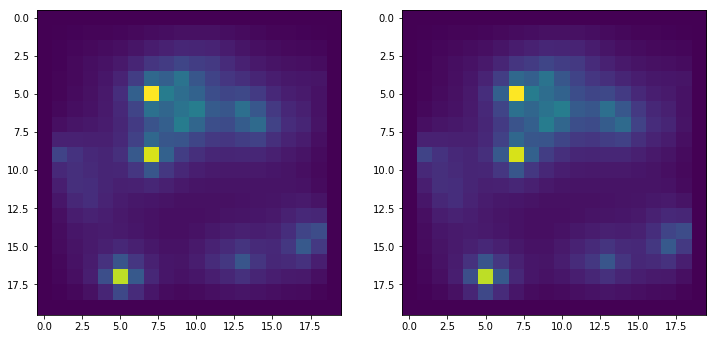
\includegraphics[width=\linewidth]{output/testcase.png}
  \caption{Comparison between result from direct solver (left) and iterative solver (right).}
  \label{fig-testcase}
\end{figure}

For this certain problem, it is obvious that iterative solver outperforms on both time and memory consumptions. As in real simulations, systems with hundreds of grid points on each dimension are commonly seen, it would be better to use iterative solver compared to the direct solver. However, it could also be seen that the iterative efficiency and accuracy both depend on Debye length ($\lambda_D$) and the requested iteration error limit, with the first one out of manual control, and the second one in need of times of trials. Therefore, although consumption of this method is lower, it might be more tricky to get the satisfying answer via this approach, especially when Debye length is considerably large.

For production problems, they are very likely to be constrained by time consumption of direct solver on first run, which grows as a speed of $O(N^3)$. Therefore before the memory exhausts, it is very likely that the computation time becomes unacceptable. For iterative solver, the major constraint is time (iteration cycle numbers), but memory cost is still worrying. However, as this is a sparse matrix, it could be saved in a much more effective way, thus eliminating the memory concerns. To make the solvers parallel, the partial-pivoting LU-decomposition method might need modifications in order to run on different cores or even nodes.

\begin{itemize}
    \item Which solver does better? (compute time, memory) Discuss why this is a better solve solver so that a non-specialist may appreciate the conclusion. 
    \item Which solver will do better for a production scale problem? Justify this conclusion.
    \item Discuss how the production problem projections will be constrained and what will need to be taken into account for parallelization
    \begin{itemize}
        \item Examples: Are you going to use too much RAM for a single node (and why is not reasonable to switch to a lower memory-use algorithm)? Is the compute time going to be unreasonable (Why is unreasonable)?
    \end{itemize}
\end{itemize}


\section{Parallelization}

For parallelation, we choose Jacobi's iterative method. The electric potential field is smashed into a vector, and the operator is changed into its matrix form, which could be written as
\[\mathbf{A\Phi}=\frac{\mathbf{\rho}}{\varepsilon}\]
The major time consumption is expected to take place during this iterative solver itself.

The parallelization method used in this project is MPI. Since the system matrix $\mathbf{A}$ could become considerably large for those product-size problems, it is a better practice to use a distributed memory method to carry out the parallelization. Also, such a method enables the possibility of running the program on distributed nodes, which means it could be executed with more computational resource and easier to scale compared to those shared memory methods.

As Jacobi iterative solver needs communications during solving to update the target vector on each process, Map-reduce is not an appropriate method for this problem. OpenMP and Threads are both shared-memory methods and are less favoured as discussed above. The iterative method could be decomposed to row-wise operations for the matrix, and during the calculation step (after which will be the updating of vector), there is no need to get access to other matrix elements located on other processes, while \texttt{MPI\_Broadcast()} is enough to take on the task of updating of the vectors, therefore there is no need to make use of global address space, which means there is no need to use PGAS method.

MPI method requires a drastic reconstruction of the original code, therefore nearly every class needs rewriting. However, the most important parallelizations are on the initialization of A matrix and the iterative solving steps. Since each process only stores part of A matrix, this could be generated in a parallel way for this program. During the iterative solving of the linear equation, we need to multiply the vector by the matrix to get the updated value, while this could be done independently for each row of vector, therefore by storing the matrix distributively, the matrix multiplication could also be parallelized, which is the most significant part of the parallelization for this certain method.

As most of the time consumption for solving takes place in Jacobi solver itself, it is possible that the percentage of parallelization is very close to 100\%, at least higher than 95\%, at first glance. However, from the following discussion on profiling of the parallel version of the code, we will find that parallelization is not a free lunch with the cost of communications between processes, especially broadcasting of data, whose time consumption can even grow as the parallelization size gets larger. A small portion of the code, such as I/O operations, are intrinsically not able to be parallelized. Besides, broadcasting the right hand side of the linear equation to every process during the initialization is also a step which could not be parallelized, though all these vector operations are typically must faster than matrix operations. For a linear system with size of $N$, this will cost around $1/N$ of total running time.

Setting up the matrix is similar to that of sequential version of program, except that now only a piece of matrix is stored on one single process, and each process only needs to generate a part of it, therefore as could be seen in the source code, in the generation of system matrix, we add conditions to jump through the loops, so that only a small portion of elements will be covered on each process. Generation of b vector (right hand side) is similar, but as this vector is stored with a complete copy on each process, we need to use broadcast after the generation. These are the obvious differences in generation of the matrix and the RHS vector.

\subsection{Profiling}

\subsubsection{Serial}

The profiling is done with a $ 20\times 20 \times 20$ grid number of 3D-field, with Dirichlet's boundary condition, therefore dimension of the linear system is 5832. The profile result for the serial code is shown as below:

\begin{figure}[H]
  \centering
  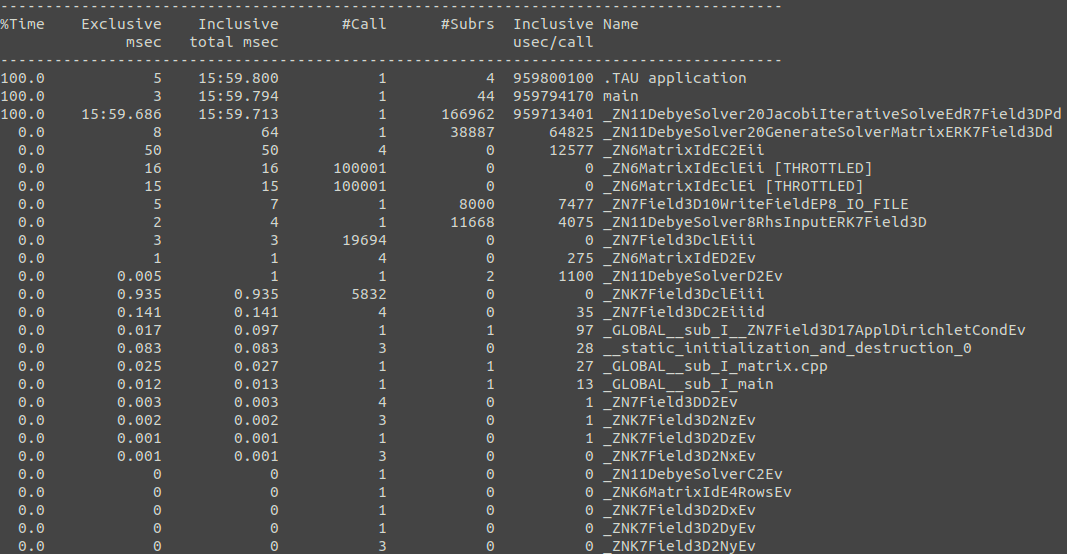
\includegraphics[width=\linewidth]{output/serial-previous-text.png}
  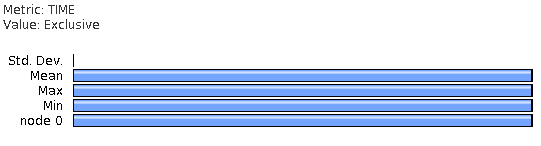
\includegraphics[width=0.6\linewidth]{output/serial-previous.png}
  \caption{The profile results of serial code.}
  \label{fig-testcase}
\end{figure}

As could be seen, nearly 100\% of time is consumed on the \texttt{JacobiIterativeSolve()} function, which is the major function of iterative solver itself. This is just the same as our expectation discussed previously.

To further study the time consuption, we take the main iteration in Jacobi solver out as a stand-alone function (\texttt{DebyeSolver::MatMul()}). This is the matrix-vector multiplication part for the iteration process. As could be seen from the new profile results, this small part, though only consisted of two lines, is still taking around 100\% of time.

\begin{figure}[H]
  \centering
  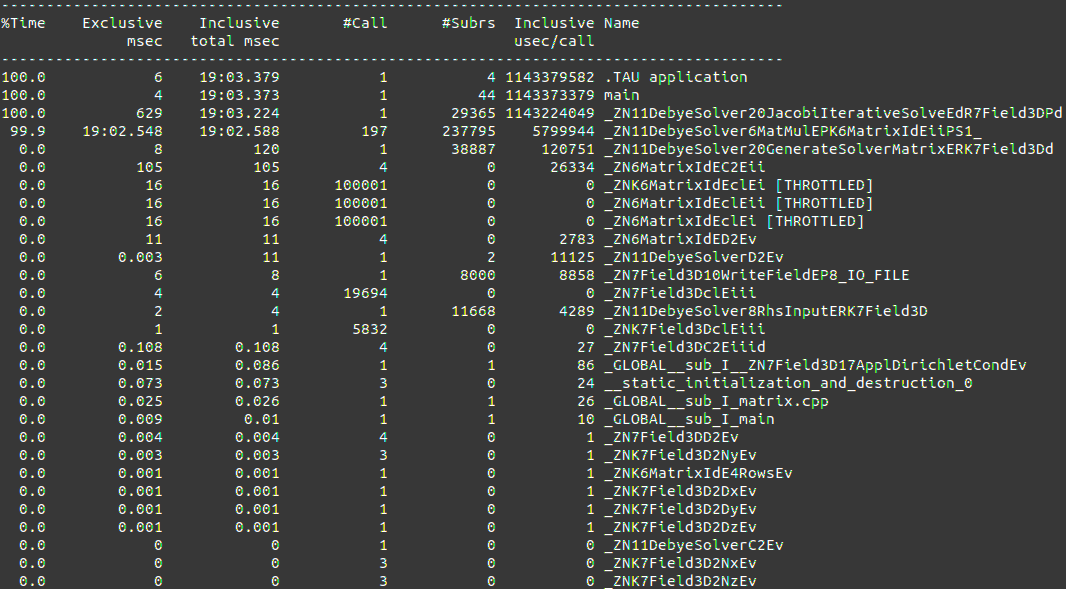
\includegraphics[width=\linewidth]{output/serial-separated-text.png}
  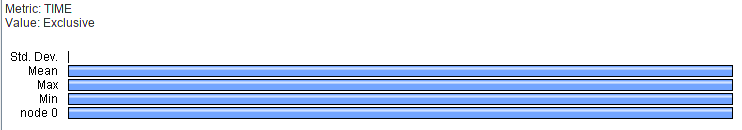
\includegraphics[width=0.6\linewidth]{output/serial-separated.png}
  \caption{The profile results of serial code with matrix-vector multiplication separated. Blue is for \texttt{MatMul()} function.}
  \label{fig-testcase}
\end{figure}

As nearly all time consumption comes from the solving of equation itself, there is no obvious and simple way to upgrade the efficiency. Here we are simply changing the compiler's flag from \texttt{-O2} to \texttt{-O3}. Other possible ways might include changing the compilers, rewriting the code to make full use of CPU cache, or try to optimize the algebraic operations to make full use of FMA.

Below is the updated profile with the new optimization flag.

\begin{figure}[H]
  \centering
  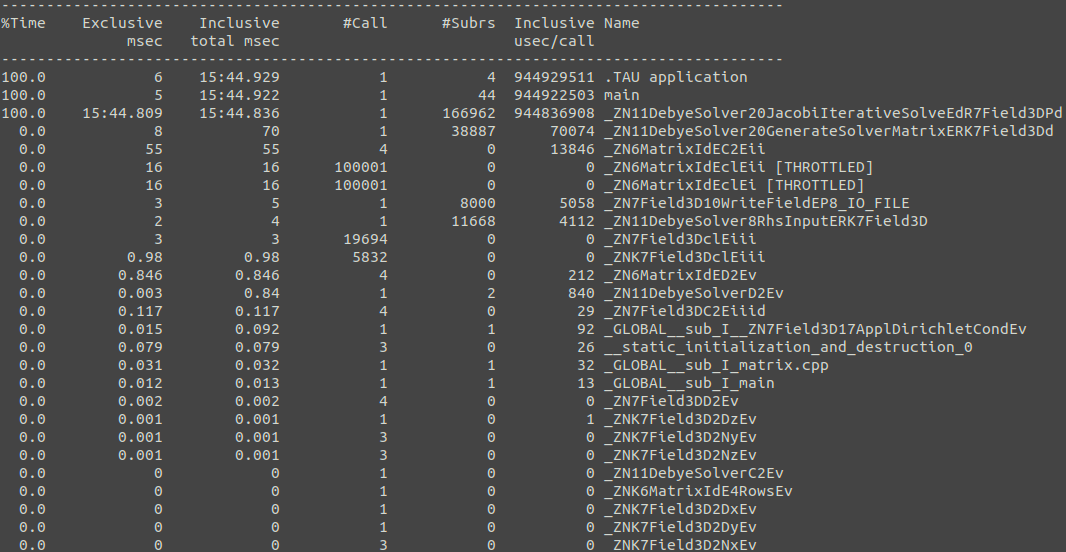
\includegraphics[width=\linewidth]{output/serial-improved-text.png}
  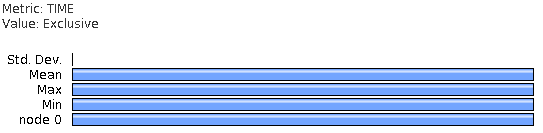
\includegraphics[width=0.6\linewidth]{output/serial-improved.png}
  \caption{The profile results of serial code with improved compiling flag.}
  \label{fig-testcase}
\end{figure}

As could be seen from the results, there is a slight improvement in the speed. For the same problem size, the time consumed decreases from 15 min 59 s to 15 min 45 s, shortened by around 1.5\%. However, this might also be influenced by other factors such as the load of server.

\subsubsection{Parallel}

The profiling is done with a $ 20\times 20 \times 20$ grid number of 3D-field (i.e., still sample size), with Dirichlet's boundary condition, therefore dimension of the linear system is 5832. The profile result for the MPI parallel version of code is shown as below, with \texttt{-np=10}:

\begin{figure}[H]
  \centering
  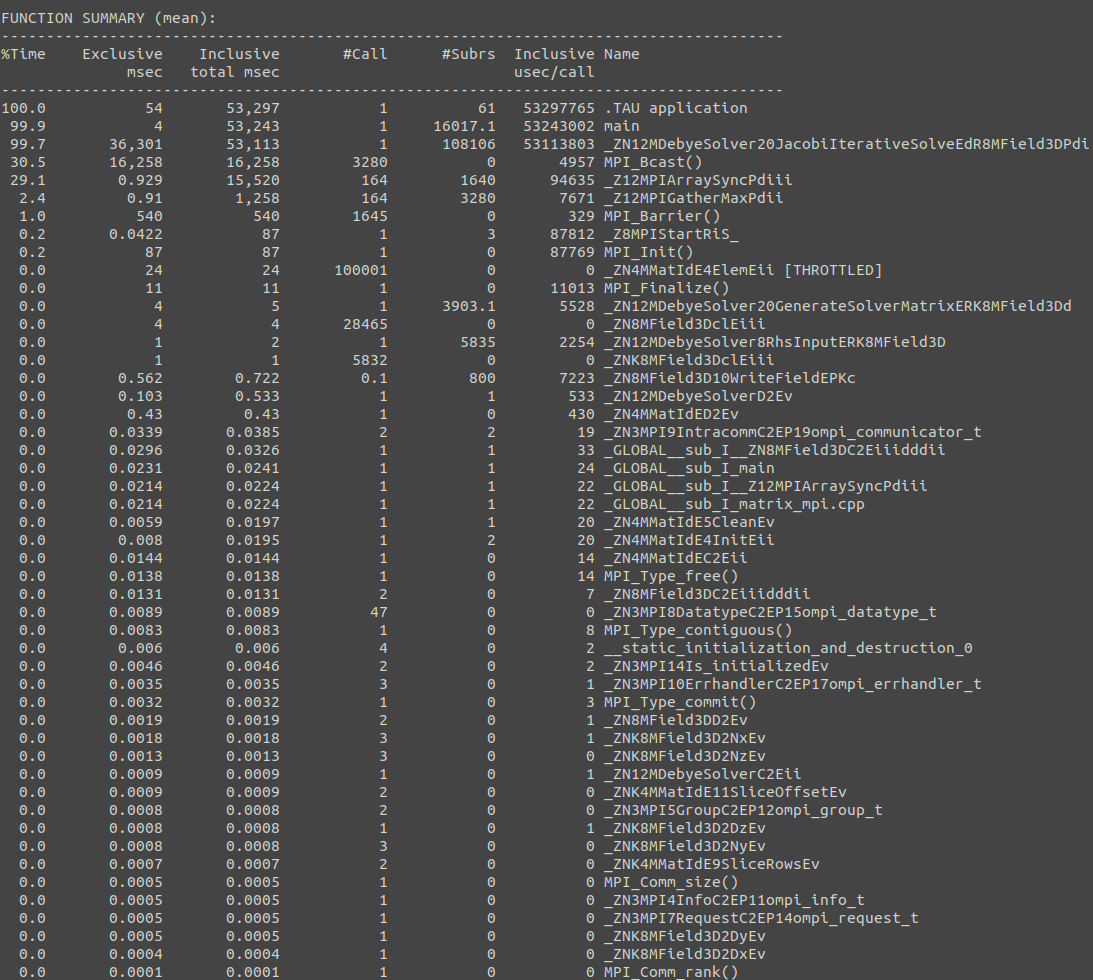
\includegraphics[width=\linewidth]{output/mpi-previous-text.png}
  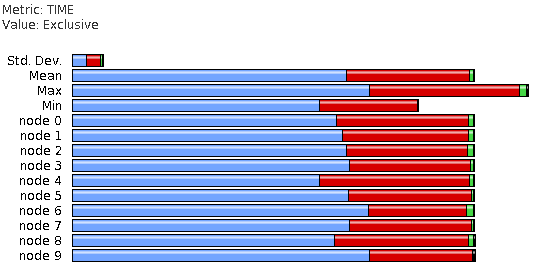
\includegraphics[width=0.6\linewidth]{output/mpi-previous.png}
  \caption{The profile results of parallel code.}
  \label{fig-testcase}
\end{figure}

As shown in the profile, the major contribution of the time consumption still comes from the algebraic operations inside of the solver itself (shown in blue). However, this time we see a significant contribution from the talk between processes, i.e., time consumption on \texttt{MPI\_Bcast()} (shown in red).

These two factors are both as expected, however, the time consumption on the talking is much higher than the initial guess, since it is obviously not at a scale of $1/N$. This might be related with specific computer architecture, or number of nodes involved (though we are only using one node here).

Similar to serial case, we then separate the matrix multiplication process from the solver routine to form a stand-alone function. Again, it is still the most time-consuming procedure in the computation.

\begin{figure}[H]
  \centering
  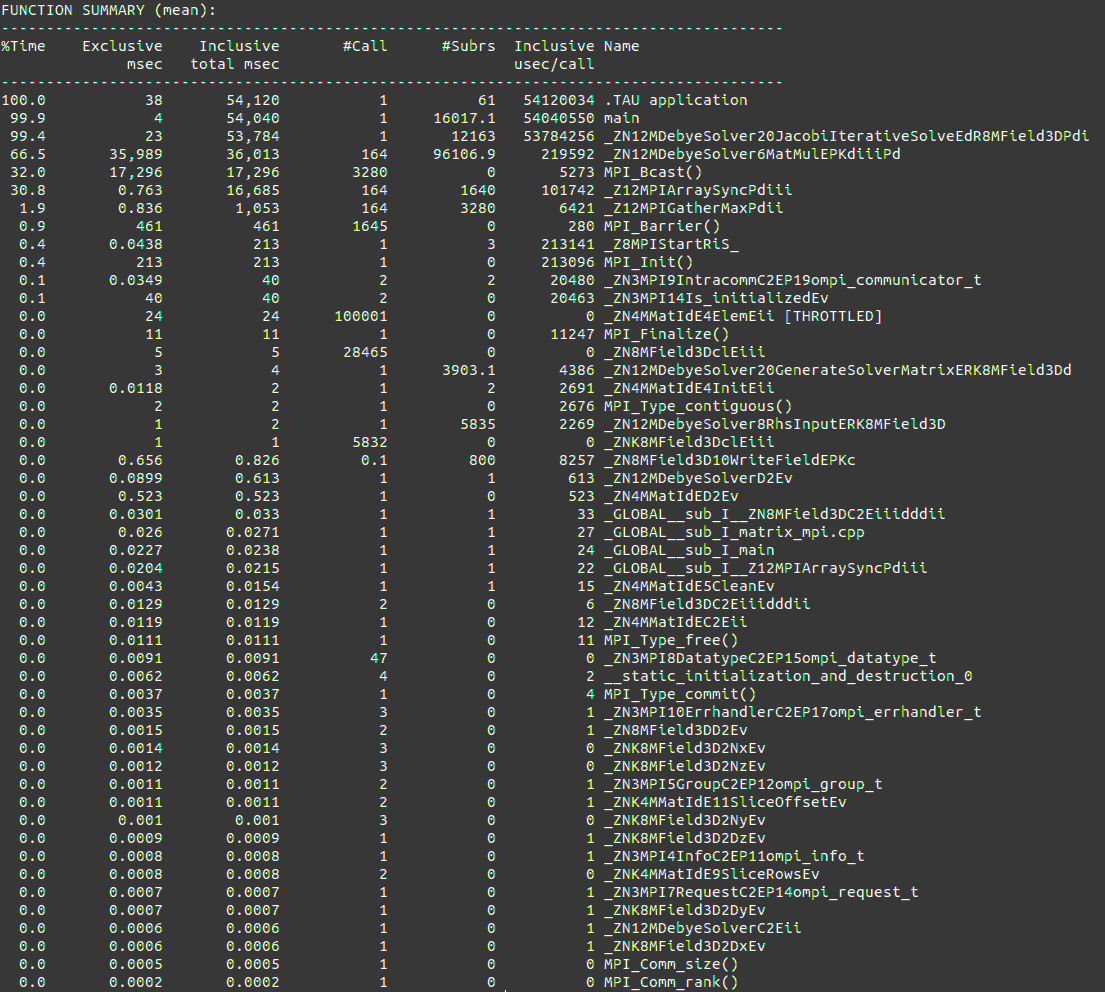
\includegraphics[width=\linewidth]{output/mpi-separated-text.png}
  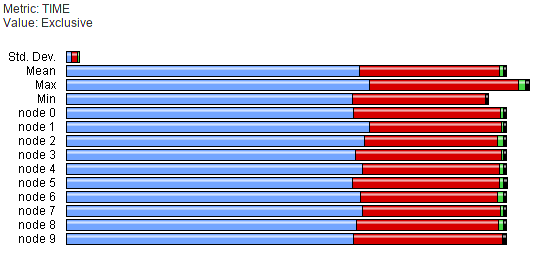
\includegraphics[width=0.6\linewidth]{output/mpi-separated.png}
  \caption{The profile results of parallel code with matrix-vector multiplication separated. Blue is for \texttt{MatMul()} function.}
  \label{fig-testcase}
\end{figure}

A direct comparison of speed could not be provided by the executable file with the profiling tool implemented, since the profile can induce noticeable difference between serial and parallel code. Here we only compare the execution time ratio of different functions for serial and parallel codes. As could be seen, the \texttt{JacobiIterativeSolve()} method is still the most time-consuming part, while at this case it is distributed onto different nodes, and the total amount of time is therefore decreasing, as expected.

Compared with the serial code in PR \#1, the parallel version of code is running with way much shorter time (the serial part of code is taken from the code in PR \#1), which could be seen from the profile results. However, the memory cost is slightly rising, since each node is now holding a complete copy of the RHS vector and solution vector. But this is not an obvious cost, since the size of matrix is thousands of times larger, while that is stored piecewise and shall not induce a strong memory increase.

As MPI communication is time-consuming for parallel code with \texttt{-np=10}, it is possible to substitute \texttt{MPI\_Bcast()} by other functions as \texttt{MPI\_Allgatherv()}, to see which has a higher efficiency. With such a modification, the profile is shown as below:

\begin{figure}[H]
  \centering
  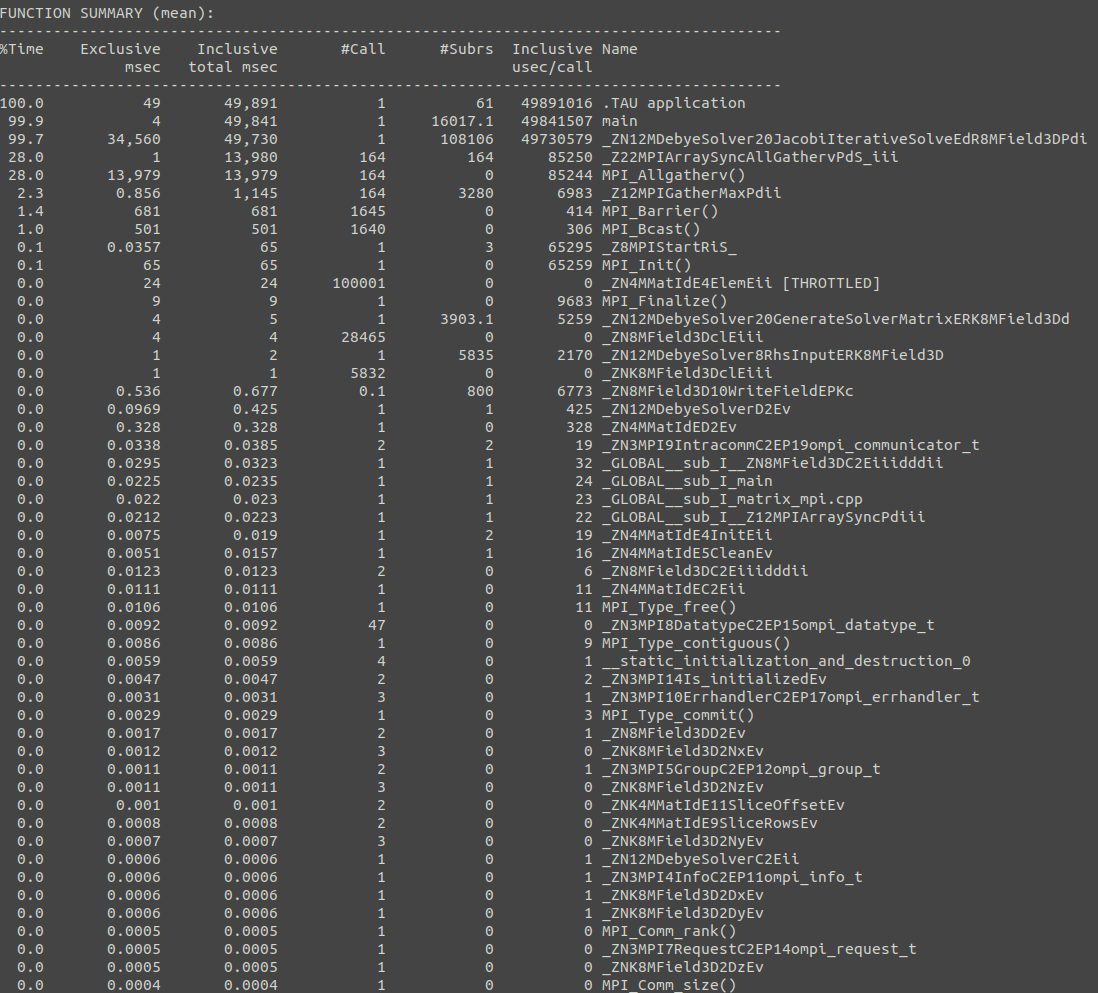
\includegraphics[width=\linewidth]{output/mpi-gather-text.png}
  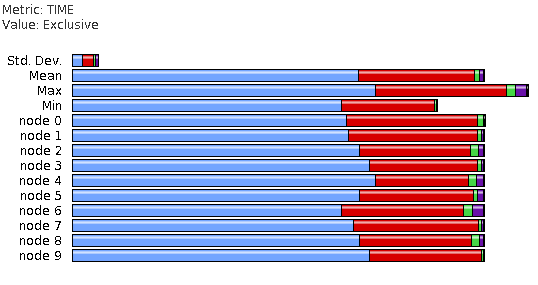
\includegraphics[width=0.6\linewidth]{output/mpi-gather.png}
  \caption{The profile results of parallel code with MPI\_Allgatherv().}
  \label{fig-testcase}
\end{figure}

After changing the MPI communication function, there is a slight accelaration in the average running time of the functions. Another way is to reduce the number of processes to no larger than number of cores on the node, see the scaling discussion below for details.

\subsection{Scaling}

The plot for execution time of strong scaling on login node of ACI is shown as below:

\begin{figure}[H]
  \centering
  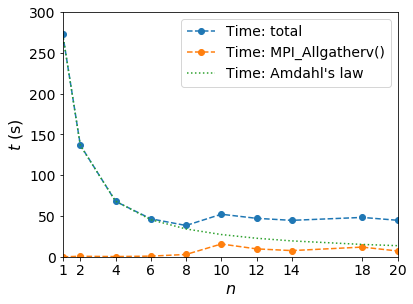
\includegraphics[width=0.5\linewidth]{output/scaling-updated.png}
  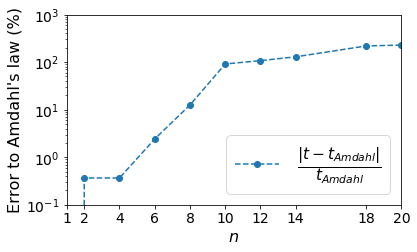
\includegraphics[width=0.5\linewidth]{output/scaling-error.png}
  \caption{The profile results of parallel code with MPI\_Allgatherv(), and the relative error of overall execution time from Amdahl's law.}
  \label{fig-testcase}
\end{figure}

The plot starts with $N=1$, which is actually serial, with the same problem size as above examples. This size is already large enough to profile the speed up of parallelization, and starting from $N=1$ makes it easy to get the expected computation time from Amdahl's law. From this plot we could also see that the number \texttt{-np=10} is actually not a good choice for the parallel code profiling example, since it gives a large overhead of communication time between processes. However, this does not influence the validity of those discussions.

From the plot, it could be seen that \texttt{-np=8} should be used for speed for the sample-sized problem, while the best efficiency is reached at \texttt{-np=1}, where no communication happens. For a research problem, more processes with an acceptable efficiency will be preferred as this might be related with the cost of computational resources, therefore \texttt{-np=8} can be used as a result of balancing between performance and efficiency, if efficiency does not vary as the size of problem grows, which needs to be further investigated by weak scaling tests. Also, the communication cost rises drastically after $N \geq 10$, which can be related with the server and node structure, and could be varying on different architectures. For this test, since the login node has 8 cores, which could be confirmed with "\texttt{cat /proc/cpuinfo}", the speed up will be limited after that number, i.e., $N > 8$. Therefore, for nodes with more cores, using more processes, such as $N=10$, might be a better choice.

If we take $p \approx 100\%$ from the profile of serial code, then Amdahl's law could be written as

\[S=\frac{t_\mathrm{serial}}{t_\mathrm{parallel}} \approx s = \min{(N_\mathrm{processes}, N_\mathrm{cores})}.\]

However, this is only possible if no communication cost, which could even arise (seen from above), is considered.

From the plot above, we can see that for $N \leq 8$, the speed is very close to ideal, but for other numbers of processes, the program is way much slower (except for the serial case, $N=1$). The reason for a lower speed with $N > 8$ is already discussed as a limit of number of cores, and for $N = 8$ the communication cost is already arising, therefore we see a small but observable deviation from the ideal expectation.

\section{Coupling to an External Library}

\subsection{Coupling}

The matrix-vector multiplication operation in Jacobi solver, i.e., the \texttt{MatMul()} function, is the most computationally intensive part of the code, which takes most of the time despite the fact that it is only a few lines. What's more, it is a typical linear algebraic problem where libraries routines could give a huge acceleration. Therefore it is necessary to replace this with an external library.

We are using Intel MKL for this specific function. The reason for choosing this library is based on the following facts:
\begin{itemize}
    \item The processors of the test environment are Intel Xeon. MKL is especially optimized for those Intel processors.
    \item Intel MKL is a high-performance library itself, whose efficiency is slightly higher than many open-source libraries.
    \item The function has a corresponding routine in MKL library, which makes it easy to implement.
    \item MKL has the interface corresponding to BLAS/LAPACK/FFTW routines, therefore it is more compatible with possible further programs.
\end{itemize}

To couple this library to the code, we use the \texttt{cblas\_dgemv()} function to carry out the matrix-vector multiplication, that is, to replace the function \texttt{MatMul()} directly with this routine. Please refer to the code (\texttt{debye\_mpi.h}) for details.

The updated profile for 10 processes is shown as below:

\begin{figure}[H]
\centering
      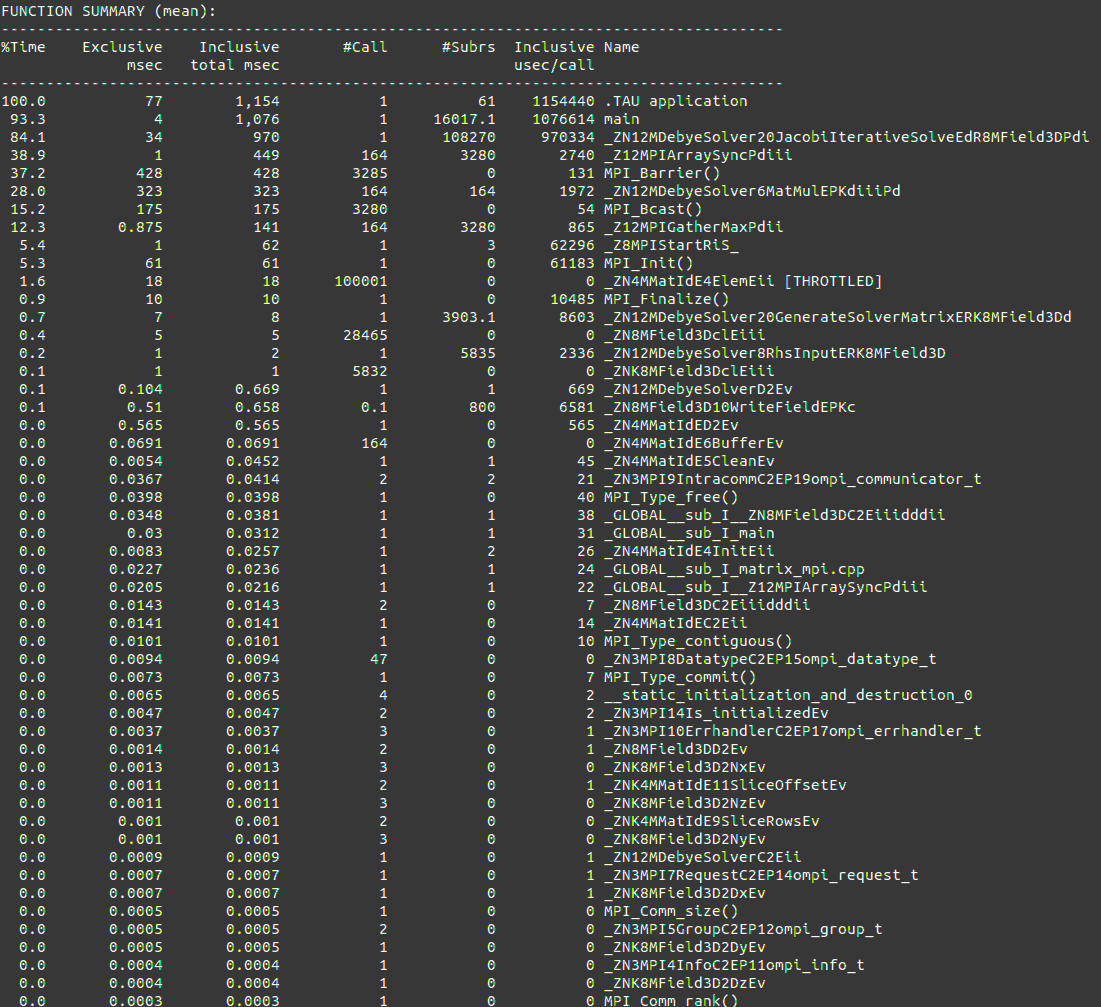
\includegraphics[width=0.8\linewidth]{output/mkl-profile-text.png}
      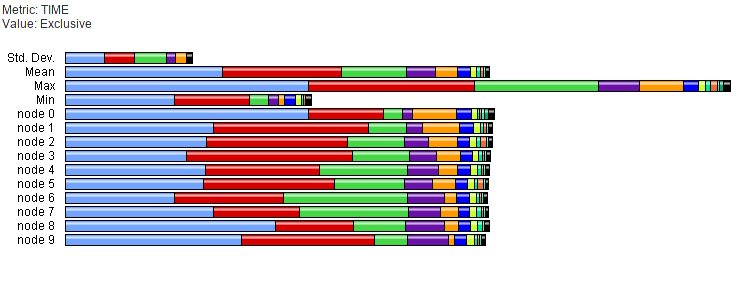
\includegraphics[width=0.8\linewidth]{output/mkl-profile.png}
  \caption{Profiling results for code with MKL. Blue part is for \texttt{MPI\_Barrier()}, red for \texttt{MatMul()}, and green for \texttt{MPI\_Bcast()}.}
\end{figure}

Compared with the previous parallel version, it could be seen that the matrix-vector multiplication now consumes way much less time: the time consumption for \texttt{MatMul()} with 10 processes is reduced from around 36 s to 0.3 s. A plot for scaling is also shown as below:

\begin{figure}[H]
\centering
      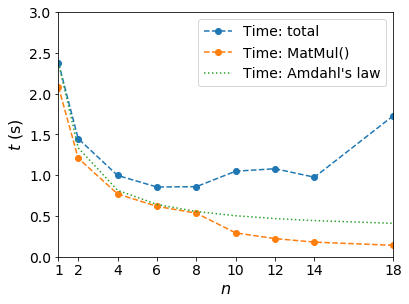
\includegraphics[width=0.5\linewidth]{output/scaling-mkl.png}
      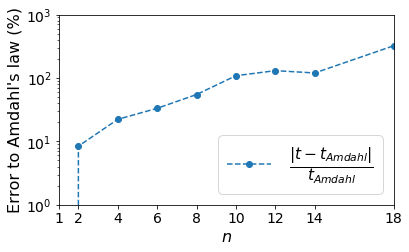
\includegraphics[width=0.5\linewidth]{output/scaling-error-mkl.png}
  \caption{Strong scaling results for code linked with MKL. The second subfigure shows the deviation from Amdahl's law.}
\end{figure}

We can directly read from this figure and the scaling result for previous sections that the total time consumption of the program is significantly lowered. Another aspect to notice is that proportion of time consumptions in other routines, especially MPI routines, are significantly increased.

\subsection{Potential Coupling}

Up till now, the core part of Jacobi iterative solver is well accelerated. However, the result output and matrix generation (matrix operations) are still not optimized. They are the parts that might also be changed to other routines from external libraries. It is, we can use I/O libraries and other linear algebraic routines to further speed up the code. The code now is not using direct solver, so matrix decomposition routines are not applicable to it. However, to speed up the direct solver, external library providing fast decomposition routines are definitely appealing. When we feel like using the direct solver for the cases where Jacobi solvers cannot be applied (e.g., does not converge), then advanced decomposition techniques can be applied.

The iterative solver uses a sparse matrix, and the iteration is related with updating the vector by only multiplying it with the off-diagonal elements in the matrix. Currently it is done by subtracting the diagonal elements after multiplication, but with sparse matrix and graph division we could also split it into operation over subsections for a graph, which provides another possibility to evaluate the updated vector.

We are already using MKL in the code, so definitely it is possible to use solver libraries. However it is does not eliminate the possiblity of implementing other solver libraries such as boost. We are not using parallel I/O library now since the data array we are dealing with is not amazingly large. But it would not be a bad idea to use parallel I/O libraries.

The most time consuming part it matrix-vector operation in this code, so accelerators are feasible for this problem. With CuBLAS or manual processing, it is possible for the code to experience tens of times of acceleration compared with its sequential partner.

Among these choices, using the accelerator might be the most worthwhile, since in MPI the portion of communication cost is is rather high after linking the solver library, and accelerator can eliminate such a cost of memory communication to a large extent if implemented in a proper way.

\section{Discussion and Conclusions}

In this report, we have discussed the physical problem to be solved, the method of discretization, the structure of the matrices/vectors to be constructed, and two different kinds of sequential solvers applied to solving of the problem.
The problem is, as stated in the first section, solving Poisson equation with Debye-Huckel's linear shielding term. The problem is of interest since it is related with the electrostatic field in the substances with free moving charges like electrolytes and plasma, and electric field computation is an important aspect for, and not limited to, the analysis of these substances.

We have analyzed and compared the performance of the solvers, leading to the result that Jacobi iterative solver would be a better choice for this certain problem on time and spatial consumptions.

For direct solver, we have seen that matrix decomposition is the most time-consuming part, and the back-solving takes much shorter time for problems with a large size. Therefore it is better than Gauss elimination method in the case we need to solve this equation for many times. For Jacobi iterative solver, we have proved its speed is satisfying, and process makes it compatible for parallel computations since there is no modification on the original array (current step) when carrying out computation on array of the next step.

We have discussed the implementation of parallel code for the iterative solver. Profile of the code as well as scaling of the code have been discussed. MPI is selected as the parallelization method because of the requirement of vector updating and communication, as well as the requirement of distributive storage of the matrix. As could be seen, the performance is still limited by the communication between processes, whether using \texttt{MPI\_Bcast()} or \texttt{MPI\_Allgatherv()}. Linking to MKL library also successfully speeds up the code, which is proved and discussed with the profiling and scaling results.

The problem focused in this program is now the modified Poisson equation with Debye-Huckel's linear correction term. However, such a correction is only valid when the energy of free carriers are significantly smaller than $k_B T$, where $k_B$ is Boltzmann's constant and $T$ is absolute temperature of the system. In general, the correction term from the free carriers can be an exponential term $\exp(\frac{q\Phi}{k_B T})$, and the function will become non-linear, while current problem is only its linear approximation. Future work might be focusing on solving of such non-linear equations, along with its parallelation and acceleration. As this is a physics related problem, it might even be possible to use quantum computing as simulated annealing to get a solution of a real physical system related to this problem.

\newpage
\begin{appendices}

\section{Acknowledgements}

The bracket notation in calling of the matrix element and the stream output operator of matrix are inspired by the grammar from linear algebra template header library named Eigen (\texttt{http://eigen.tuxfamily.org}). The author appreciates these notations making debugging for serial version of code a more concise process.

The author referred to the Intel MKL online documentation during the step of linking the solver to external library. The documentation was detailed and really helpful in this step.

The lecturers, graders and classmates of this course are enthusiastic and well-prepared for discussions. The author enjoys the time spent with them and appreciates the help he has received.

\section{Code}

The readers could find the code on Github with the username \texttt{sunnyssk}, under the archive \texttt{CSE597-hw3}.

\subsection{Serial Solvers}

The serial code for direct and iterative solvers are in the folder "direct-and-iterative". The source code is inside of \texttt{src} folder, which contains:

\begin{itemize}
    \item \texttt{matrix.h} - Header for matrix class, providing the matrix computation and LU decomposition functions.
    \item \texttt{matrix.cpp} - Source file containing definitions of matrix operations.
    \item \texttt{debye.h} - Declarations of electrostatic function solvers with Debye shielding.
    \item \texttt{debye.cpp} - Definitions of electrostatic solvers.
    \item \texttt{meminfo.h} - Declarations of functions for memory info output.
    \item \texttt{meminfo.cpp} - Definitions of functions for memory info output.
    \item \texttt{main.cpp} - Main entrance of the program. Calls both the direct and iterative solvers.
\end{itemize}

The compile options are listed in Makefile under root directory. Please follow the compile instructions in \texttt{Readme.md} to get the correct version of program. Make sure you have \texttt{-std=c++11} or larger in the compilation options so that \texttt{nullptr} notation is supported by the compiler. To run the program, specify the input filename after the program's name, in the following form:

\texttt{./bin/main ./input/size.txt}

The input file should contain only one line specifying number of grid points on three dimensions ($n_x$,$n_y$,$n_z$). Please be careful that the direct solver could get slow when all three numbers are larger than 20 (which means, there will be more than around 8000 points in the system).

After running the program, the solution of fields will be saved into output folder. If you would like to keep a record of the on-screen tracking information, please use output reorientation. The reader could run this program directly on ACI logon node with basic gcc support.

\subsection{Iterative Solver: Parallelation}

Under the root of archive, we have the "iterative-sequential" and "iterative-mpi" folder, storing the serial and parallel version of the code. Also there is an iPython-notebook for visualizing the results of electric potential. 

For serial version, source files are under \texttt{src} sub-folder, with \texttt{matrix.cpp} and \texttt{matrix.h} containing the matrix class, \texttt{debye.cpp} and \texttt{debye.h} containing the linear solver class, as well as the field container class, and \texttt{main.cpp} as the entrance calling the solver.

For parallel version, the structure of source file is pretty much the same, except that we are now using \texttt{\_mpi} in the filenames, and there are some MPI functions defined in \texttt{mpi\_util.cpp}.

The instructions could be found in \texttt{iterative-instructions.md} under the root of archive. Please check out there.

\subsection{Code with MKL linking}

Under the root of archive, we have the "mpi-withmkl" folder, storing the parallel version of the code with MKL routine. The source files are under \texttt{src} sub-folder, with \texttt{matrix.cpp} and \texttt{matrix.h} containing the matrix class, \texttt{debye.cpp} and \texttt{debye.h} containing the linear solver class, as well as the field container class, and \texttt{main.cpp} as the entrance calling the solver.

For parallel version, the structure of source file is pretty much the same, except that we are now using \texttt{\_mpi} in the filenames, and there are some MPI functions defined in \texttt{mpi\_util.cpp}.

The instructions could be found in \texttt{Readme.md} under the root of archive. Please check out there.

To reproduce the profile results, please use \texttt{tau} as the profiler. Due to differences in the performance of each node, it could be possible that one gets different results from that described in this report, but the tendency should be the same.

On ACI-b logon servers, you could compile and run the code directly.

\section{Poster - separate document}

Please see the poster folder for the poster file.


\end{appendices}


\bibliographystyle{acm}
\bibliography{finalReport}

\end{spacing}

\end{document}

%%%%%%%%%%%%%%%%%%%%%%%%%%%%%%%%%%%%%%%%%%%%%%%%%%%%%%%%%%%%%}}
